\documentclass[12pt,a4paper]{article}
\usepackage[utf8]{inputenc}
\usepackage[english,russian]{babel}
\usepackage{amssymb,amsfonts,amsmath,cite,enumerate,float,indentfirst}
\usepackage{graphicx}
\usepackage{geometry}
\usepackage{systeme}
\usepackage{amsmath}
\usepackage[bottom]{footmisc}
\usepackage{hyperref}
\usepackage{url}

\hypersetup{
	colorlinks,
	citecolor=black,
	filecolor=black,
	linkcolor=black,
	urlcolor=black
}
\geometry{left=2cm}
\geometry{right=1.5cm}
\geometry{top=2cm}
\geometry{bottom=2cm}


\begin{document}
    \begin{titlepage}
		\begin{center}		
			\vfill	
			Санкт-Петербургский политехнический университет \\
			Петра Великого\\
			\vskip 1cm
			Высшая школа прикладной математики и вычислительной физики \\
			Кафедра «Прикладная математика и информатика»
			\vfill
			\textbf{Отчёт\\
				по лабораторной работе №4\\
				по дисциплине\\
				«Интервальный анализ»\\}
			\vfill
		\end{center}
		\vfill
		\hfill
		\begin{minipage}{0.4\textwidth}
			Выполнил студент:\\
			Лапотников Павел Вадимович\\
			группа: 5030102/90201\\
		\end{minipage}
		\vfill
		\hfill 
		\begin{minipage}{0.4\textwidth}
			Проверил:\\
			к.ф.-м.н., доцент\\
			Баженов Александр Николаевич\
		\end{minipage}
		\vfill
		\hfill 
		\begin{center}
			Санкт-Петербург\\2022 г.
		\end{center}
	\end{titlepage}
    	
    	\tableofcontents
    	\listoffigures
    	\pagebreak
\section{Постановка задачи}
Дана линейная задача построения регресии 

\begin{equation}\label{lin_problem}
    \mathbf{y}=X\beta
\end{equation}

Для данной задачи задать набор входных и выходных значений: точечный $x$ и интервальный $y$. Необходимо провести вычисления и привести иллюстрации:
\begin{itemize}
    \item Построить информационное множество решений $\beta$, сделать точечные оценки параметров
    \item Построить коридор совместных зависимостей
    \item Задать набор предсказания внутри и вне $x$, построить набор значений выходной переменной $\mbf{y}$
\end{itemize}

\section{Теория}

\subsection{Точечная оценка параметров регрессии}
Пусть x - номер измерения в выборке, а y - получившийся результат. Тогда мы можем представить линейную регрессию как 
\[ y = b_0 + b_1*x\]
Для получения точечной оценки можно поставить задачу оптимизации

\begin{equation}
    \begin{cases}
    mid(y_i) - \omega_i * rad(y_i) \leq X*\beta \leq mid(y_i) + \omega*rad(y_i)  \quad     i=1,m \\
     \sum_{i=1}^{m} \omega_i \to  min \\
    w_i \geq 0 \\
    w, \beta = ?
    
      
    \end{cases}\,.
\end{equation}


Здесь X - матрица m x 2, в первом столбце которой элементы, равны 1, а во втором - значения $x_i$. В качестве значений середины и радиуса возьмем $mid(y_i) = y_i$ и $rad(y_i) = 1$

\subsection{Информационное множество}
Интервальное множество решений $\beta$, которое необходимо построить и оценить в задаче (\ref{lin_problem}), называется информационным множеством. \\
Построим визуальное представление информационного множества параметров $b_0$ и $b_1$. Для этого воспользуемся следующим алгоритмом:
\begin{itemize}
    \item Для индекса i от 0 до m:
    \begin{itemize}
        \item Для индекса j от i+1 до m:
        \begin{itemize}
            \item По $ (x_i, y_i \pm \epsilon)$ и $ (x_j, y_j \pm \epsilon)$ построим 4 прямые.
            \item Для каждой прямой проверим, попадает ли она во все интервалы нашей выборки
            \item Если да - сохраняем параметры прямой как вершину нашего информационного множества.
        \end{itemize}
    \end{itemize}
\end{itemize}

\subsection{Коридор совместных зависимостей}
Коридором совместных зависимостей называется множество, образованное всеми решениями с параметрами из информационного множества

\subsection{Предсказание значений}
Для предсказания значения строится сечение коридора совместных зависимостей в указанных точках

\section{Реализация}
Лабораторная работа выполнена с помощью встроенных средств языка программирования Python с использованием библиотек matplotlib, intvalpy, numpy, scipy, statsmodels в среде разработки Jupyter Notebook.

\section{Результаты}

\begin{figure}[H]
    \centering
    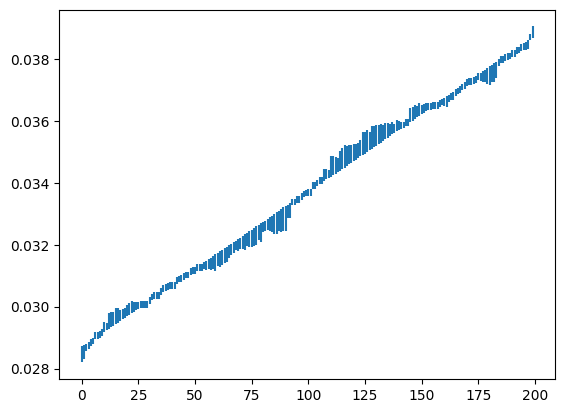
\includegraphics[width=14cm]{4_1.png}
    \caption{График входных интервальных данных}
    \label{fig:info}
\end{figure}

\begin{figure}[H]
    \centering
    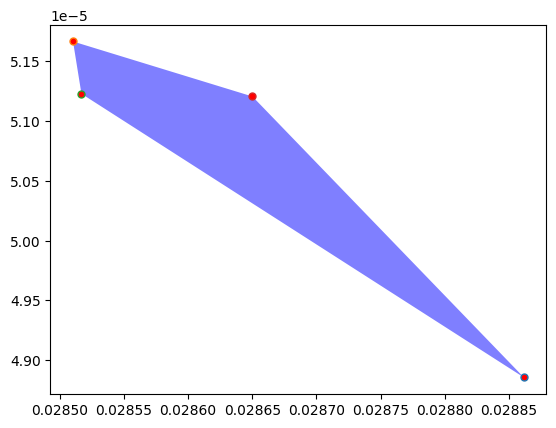
\includegraphics[width=14cm]{4_2.png}
    \caption{Информационное множество}
    \label{fig:info}
\end{figure}

\begin{figure}[H]
    \centering
    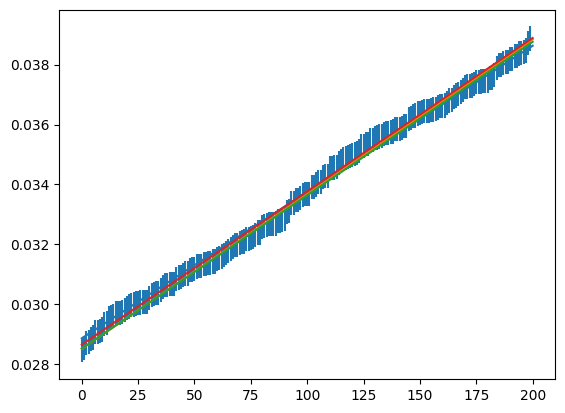
\includegraphics[width=14cm]{4_3.png}
    \caption{Допусковый корридор}
    \label{fig:info}
\end{figure}

\begin{figure}[H]
    \centering
    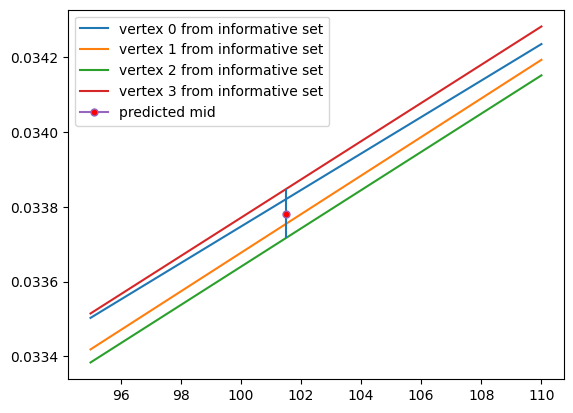
\includegraphics[width=14cm]{4_4.png}
    \caption{График построенной модели с предсказанием при аргументе 101.5}
    \label{fig:info}
\end{figure}

\begin{figure}[H]
    \centering
    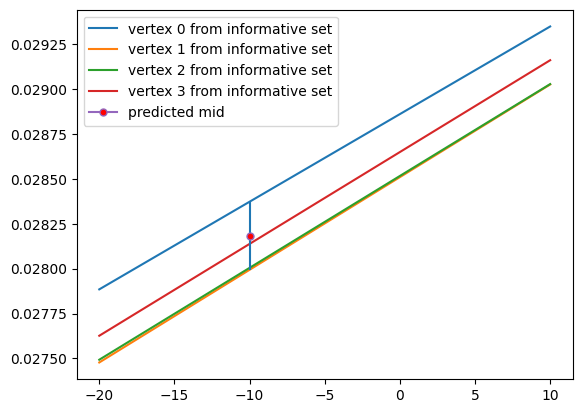
\includegraphics[width=14cm]{4_5.png}
    \caption{Предсказание значения при аргументе -10}
    \label{fig:info}
\end{figure}

\begin{figure}[H]
    \centering
    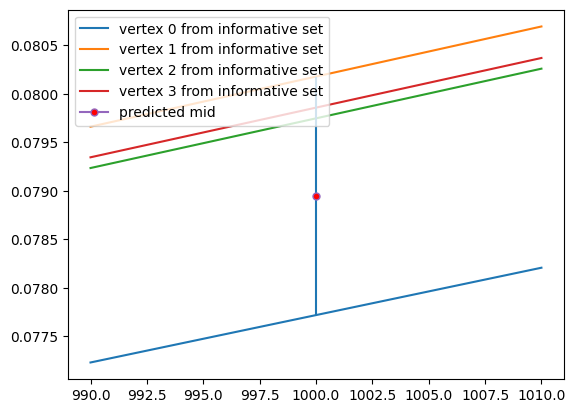
\includegraphics[width=14cm]{4_6.png}
    \caption{Предсказание значения при аргументе 1000}
    \label{fig:info}
\end{figure}


\section{Обсуждение}
\begin{enumerate}
    \item Исходя из предсказанных значений можно заметить, что при экстаполяции погрешность гораздо больше чем при интерполяции.
    \item Из предсказанных значений можно заметить, что при экстаполяции погрешность увеличивается по мере удаления от имеющихся данных.
\end{enumerate}

\end{document}
